\begin{frame}{El gasto primario alcanzó 19,9\% del PIB en 2025}
\centering
\resizebox{0.90\textwidth}{!}{
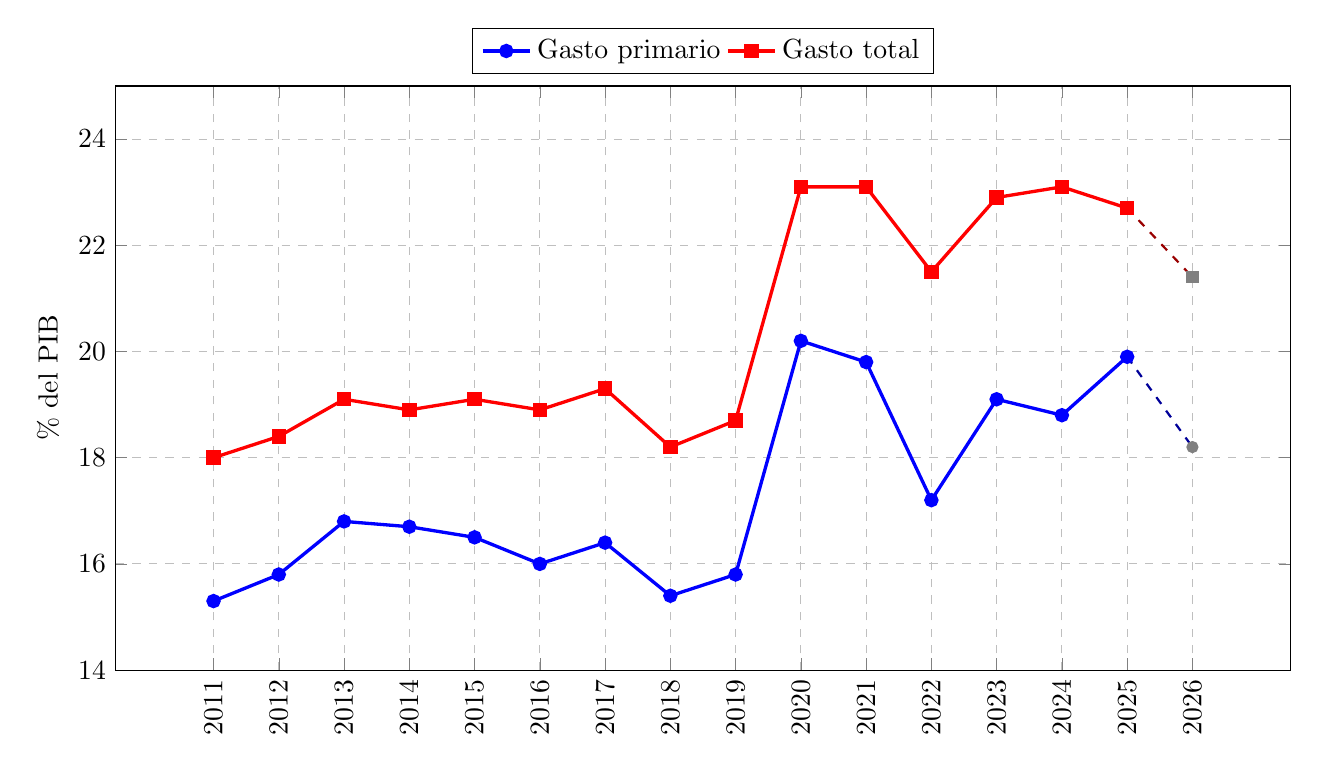
\begin{tikzpicture}
\begin{axis}[
    width=16.5cm,
    height=9cm,
    ylabel={\% del PIB},
    xtick={7,8,...,22},
    xticklabels={2011,2012,2013,2014,2015,2016,2017,2018,2019,2020,2021,2022,2023,2024,2025,2026},
    x tick label style={rotate=90,anchor=east},
    ymin=14,
    ymax=25,
    grid=both,
    grid style=dashed,
    legend style={at={(0.5,1.02)},anchor=south,legend columns=-1}
]
\addplot[color=blue,mark=*,very thick] coordinates {
    (7,15.3) (8,15.8) (9,16.8) (10,16.7) (11,16.5) (12,16.0)
    (13,16.4) (14,15.4) (15,15.8) (16,20.2) (17,19.8) (18,17.2)
    (19,19.1) (20,18.8) (21,19.9)
};
\addlegendentry{Gasto primario}
\addplot[color=red,mark=square*,very thick] coordinates {
    (7,18.0) (8,18.4) (9,19.1) (10,18.9) (11,19.1) (12,18.9)
    (13,19.3) (14,18.2) (15,18.7) (16,23.1) (17,23.1) (18,21.5)
    (19,22.9) (20,23.1) (21,22.7)
};
\addlegendentry{Gasto total}
\addplot[color=blue!60!black,dashed,thick] coordinates {(21,19.9) (22,18.2)};
\addplot[color=red!60!black,dashed,thick] coordinates {(21,22.7) (22,21.4)};
\addplot[color=gray,mark=*,only marks] coordinates {(22,18.2)};
\addplot[color=gray,mark=square*,only marks] coordinates {(22,21.4)};
\end{axis}
\end{tikzpicture}}
\scriptsize Línea sólida: resultados observados hasta 2025. Línea discontinua: proyección 2026.
\note{[Sources] MFMP 2026, capítulo 1, tablas 1.3 y 1.5. Serie histórica previa: MHCP, como en la versión fuente.}
\end{frame}